\documentclass[a4paper,12pt, oneside]{book}

%Pacchetti utili
%************
%* packages *
%************

%Codifica
\usepackage[utf8]{inputenc}

%Lingua, sostituire italian con english nel caso in cui la tesi sia scritta in inglese
\usepackage[english]{babel}

%Pacchetto per definire layout di pagina
\usepackage{fancyhdr}
\usepackage{sectsty}
\usepackage[margin=2.5cm]{geometry}

%Spazia linee all'interno del documento
\usepackage{setspace}

%Listati di codice
\usepackage{verbatim}
\usepackage{listings}

%Didascalie immagini
\usepackage[hang,small,sf,font=scriptsize, labelfont=bf]{caption}
\usepackage{subcaption}

%Inclusione immagini
\usepackage{graphicx}

%Impostazioni note a piè pagina
\usepackage[stable]{footmisc}

%Citazioni e riferimenti a label
\usepackage{cite}
\usepackage[english]{varioref}

%Colori
\usepackage[usenames]{color}
\usepackage{xcolor}
\usepackage{colortbl}

%Crea link ipertestuali
\usepackage[hidelinks]{hyperref}

%Formattazione url
\usepackage{url}

%Inserimento formule
\usepackage{amsmath}
\usepackage{mathrsfs}

%Inserimento pseudocodice
\usepackage{algorithm}
\usepackage{algpseudocode}

%Citazione frasi
\usepackage{csquotes}

%Inserimento di Lorem ipsum nel testo
\usepackage{lipsum}

%\usepackage{lmodern}



%Nuovi comandi
%*****************
%* nuovi comandi *
%*****************

\newcommand{\abs}[1]{\left|#1\right|}                               % modulo
\newcommand{\dato}{\left|\right.}                                   % probabilit\`{a} condizionata
\newcommand{\fun}[1]{\mathrm{#1}}                                   % stile funzione
\newcommand{\imp}{\;\;\Longrightarrow\;\;}                          % implicazione
\newcommand{\norma}[1]{\left\| #1 \right\|}                         % norma
\newcommand{\prob}[1]{\mathrm{P}\!\left[#1\right]}                  % probabilit\`{a}
\newcommand{\expect}[1]{\mathrm{E}\!\left[#1\right]}                % aspettazione
\newcommand{\sse}{\;\;\Longleftrightarrow\;\;}                      % se e solo se
\newcommand{\vect}[1]{{\boldsymbol{\mathrm{#1}}}}                   % stile vettore
\newcommand{\real}[1]{\fun{Re}\left[#1\right]}                      % parte reale
\newcommand{\imag}[1]{\fun{Im}\left[#1\right]}                      % parte immaginaria
\newcommand{\Dim}[1]{\fun{dim}\left[#1\right]}                      % dimensione di una matrice
\newcommand{\Det}[1]{\fun{det}\left[#1\right]}                      % determinante di una matrice
\newcommand{\Ker}[1]{\fun{ker}\left[#1\right]}                      % ker di una matrice
\newcommand{\rango}[1]{\fun{rango}\left[#1\right]}                  % rango di una matrice
\newcommand{\scalare}[2]{\left\langle #1, #2 \right\rangle}         % prodotto scalare
\newcommand{\blbrace}{\left  \lbrace}                               % parentesi graffa sinistra grande
\newcommand{\brbrace}{\right \rbrace}                               % parentesi graffa destra grande
\newcommand{\sinc}{\fun{sinc}}                                      % sinc
\newcommand{\rect}{\fun{rect}}                                      % rect
\newcommand{\rcos}{\fun{rcos}}                                      % rcos
\newcommand{\sgn}{\fun{sgn}}                                        % sgn
\newcommand{\N}{\mathbb{N}}                                         % insieme dei numeri naturali
\newcommand{\Z}{\mathbb{Z}}                                         % insieme dei numeri interi
\newcommand{\Q}{\mathbb{Q}}                                         % insieme dei numeri razionali
\newcommand{\R}{\mathbb{R}}                                         % insieme dei numeri reali
\newcommand{\C}{\mathbb{C}}                                         % insieme dei numeri complessi
\newcommand{\seq}[2][n]{#2_{0}, #2_{1}, \ldots, \, #2_{#1}}         % sequenza
\newcommand{\Span}[2][n]
{\fun{span} \blbrace #2_{1}, #2_{2}, \ldots, \, #2_{#1} \brbrace}   % spazio generato
\newcommand{\ddt}{\frac{\fun{d}}{\fun{dt}}}                         % derivata
\newcommand{\Div}[2]{#1 \; \mid \; #2}                              % divide
\newcommand{\MCD}[2]{\fun{MCD}\(#1, #2\)}                           % massimo comun divisore
\newcommand{\mcm}[2]{\fun{mcm}\(#1, #2\)}                           % minimo comune multiplo
\newcommand{\goodgap}{
                      \hspace{\subfigtopskip}
                      \hspace{\subfigbottomskip}
                     }                                              % interlinea opportuna per le sottofigure
\newcommand{\eng}[1]{\emph{#1}}                                   % inglese
\newcommand{\virg}[1]{``#1"}                                        % fa una citazione tra virgolette
%\newcommand{\unit}[2]($\frac{\text{#1}}{\text{#2}}$)                % unit\`{a} di misura
\newcommand{\textttvar}[1]{{\ttvar #1}}

\definecolor{gray}{gray}{0.9}
\newcommand{\listato}[1]{\lstset{language=#1, numbers=left, numberstyle=\tiny, stepnumber=2, numbersep=5pt, numberblanklines=false, xleftmargin=5pt, captionpos=b, stringstyle=\ttfamily, columns=flexible, showstringspaces=false, tabsize=2, frame=single, framerule=0pt, backgroundcolor=\color{gray}, basicstyle=\small}}

%****************************
%* ridefinizioni di comandi *
%****************************

\renewcommand{\(}{\left(}                                     % parentesi tonda sinistra grande
\renewcommand{\)}{\right)}                                    % parentesi tonda destra grande
\renewcommand{\[}{\left[}                                     % parentesi quadra sinistra grande
\renewcommand{\]}{\right]}                                    % parentesi quadra destra grande
\renewcommand{\exp}[1]{\fun{e}^{#1}}                          % esponenziale
\renewcommand{\gcd}[2]{\fun{gcd}\(#1, #2\)}                   % massimo comun divisore

\renewcommand{\lstlistingname}{Listing}
\renewcommand{\lstlistlistingname}{Elenco dei listati codice}

\makeatletter
\def\BState{\State\hskip-\ALG@thistlm}
\makeatother

%Definizione input e output pseudocodice
\renewcommand{\algorithmicrequire}{\textbf{Input:}}
\renewcommand{\algorithmicensure}{\textbf{Output:}}
 
%"Nome" della bibliografia
\addto{\captionsenglish}{%
  \renewcommand{\bibname}{References}
}

%Impostazioni dei margini, definizione di colori e di stili vari
\newfont{\ttvar}{cmvtt10 scaled 1200}     % nuovo carattere tipi courier a spaziatura variabile per le dimostrazioni

% margini senato
%\textwidth       =  14.50 cm            % larghezza 21 cm - 4 cm (sinistro) - 2.5 (destro)
%\textheight      =  23.10 cm            % altezza 29.7 cm - 3 cm (superiore) - 2 (inferiore)
%\topmargin       =   0.00 cm            % margine superiore 3 cm diminuito di 1 inch
%\oddsidemargin   =   1.46 cm            % margine sinistro 4 cm diminuito di 1 inch
%\evensidemargin  =  -0.04 cm            % margine destro 2.5 cm diminuito di un inch

\setlength{\headsep}{1.0cm}
\setlength{\footskip}{1.0cm}
\parindent = 0.7cm
\captionmargin = 0.7cm

%Interlinea 1.5
\onehalfspacing

% stile pagina
\pagestyle{fancy}
\renewcommand{\chaptermark}[1]{\markboth{\chaptername\ \thechapter.\ #1 }{}}
\renewcommand{\sectionmark}[1]{\markright{\thesection\ #1}{}}
\fancyhead{}
\fancyhead[LE,RO]{\sffamily \thepage}
\fancyhead[RE]{\sffamily \leftmark}
\fancyhead[LO]{\sffamily \rightmark}
\fancyfoot{}

% ridefinisco lo stile plain
\fancypagestyle{plain}{ \fancyhead{} \fancyfoot{}
\fancyfoot[C]{\sffamily \thepage}
\renewcommand{\headrulewidth}{0pt}}

% stile per i titoli
\allsectionsfont{\sffamily \raggedright}

% definisco i colori
\definecolor{codegreen}{rgb}{0,0.6,0}
\definecolor{codegray}{rgb}{0.5,0.5,0.5}
\definecolor{codepurple}{rgb}{0.58,0,0.82}
\definecolor{backcolour}{rgb}{0.95,0.95,0.92}
\definecolor{backcolourwhite}{rgb}{1,1,1}

%definisco stile listati di codice
\lstdefinestyle{mystyle}{
    backgroundcolor=\color{backcolour},   
    commentstyle=\color{codegreen},
    keywordstyle=\color{magenta},
    numberstyle=\tiny\color{codegray},
    stringstyle=\color{codepurple},
    basicstyle=\ttfamily\footnotesize,
    breakatwhitespace=false,         
    breaklines=true,                 
    captionpos=b,                    
    keepspaces=true,                 
    numbers=left,                    
    numbersep=5pt,                  
    showspaces=false,                
    showstringspaces=false,
    showtabs=false,                  
    tabsize=2
}

\lstset{style=mystyle}
\lstset{emph={RandomForestClassifier, RandomizedSearchCV, GridSearchCV},emphstyle=\underbar}



\begin{document}

\begin{titlepage}
\begin{center}

\includegraphics[scale=0.1]{images/logo.png}\\

%Per il frontespizio del dipartimenti di Ing. dell'Informazione commentare le riga precedente e decommentare la successiva
%
\includegraphics[scale=0.2]{images/logo_unipd.png} \hfill 
\includegraphics[scale=0.2]{images/logo_dei.png}\\
\vspace{0.8cm}
\textsc{\LARGE University of Padua}\\
\vspace{0.45cm}
\textsc{\large Information Engineering Department}\\
\vspace{0.4cm}
\textsc{\large Master’s Degree in Computer Engineering}\\
\vfill
% Title
{ \LARGE \bfseries Solutions to the Travelling Salesman Problem
}\\
\vfill
\textit{\large Professor:} \hfill \textit{\large Student:}\\
\textsc{\large Prof. Matteo Fischetti} \hfill \textsc{Thomas Porro}\\
\hfill \textsc{1237030}\\

\vfill
% Bottom of the page
{\large Academic year 2021/2022}
\end{center}
\end{titlepage}

%\thispagestyle{empty} %pagina bianca dopo il titolo
%\cleardoublepage

\pagenumbering{roman} %numerazione romana per l'indice, l'abstract e i ringraziamenti
\thispagestyle{empty}

%\clearpage{\pagestyle{plain}\cleardoublepage}
%%definisco il layout dell'abstract
\def\changemargin#1#2{\list{}{\rightmargin#2\leftmargin#1}\item[]}
\let\endchangemargin=\endlist 

%Genero l'ambiente per l'abstract
\newcommand\summaryname{Abstract}
\newenvironment{Abstract}%
    {\begin{center}%
    \bfseries{\summaryname} \end{center}}
    
\begin{Abstract}
\begin{changemargin}{1cm}{1cm}
Inserire abstract. I margini nell'abstract sono stati ridotti di un centimetro. In caso non si volesse questa riduzione rimuovere \textit{changemargin}.
\end{changemargin}
\end{Abstract}

%\clearpage{\pagestyle{plain}}\cleardoublepage}
\tableofcontents %Indice

\clearpage{\pagestyle{plain}\cleardoublepage} %Numerazione araba per i capitoli
\pagenumbering{arabic}


%\clearpage{\pagestyle{plain}\cleardoublepage} %Comando per iniziare il capitolo su pagina dispari
\chapter{Introduction} %Nome capitolo
\label{chapter:primo_capitolo} %Label per creare riferimenti al capitolo
In this report I am going to describe, analyze and implement solutions for the Travelling Salesman Problem (hereafter referred to as TSP).\\
The TSP is a NP-hard problem formulated as follows:
\begin{displayquote}
	\textit{Given a list of cities and the distances between them, find the shortest path that connects all the cities and return to the origin one.}
\end{displayquote}
It is used mainly in plain logistics, planning, and as a benchmark for
testing optimization problems. However, it can be helpful in many other
areas with a slight modification of the formula - such as in DNA sequencing,
considering cities as DNA fragments, and astronomy, where they are stars.\\
Even though it is an NP-hard problem, instances with the dimensions of thousand or even millions of cities can be solved  with great precision (around 1\%) thanks to many heuristics and exact algorithms.

\section{Brief history of the problem}
The German handbook \textit{Der Handlungsreisende} from 1832 was a guide
used by salesman traveling through Germany and Switzerland. Albeit
without any mathematical languages, it proves that people were starting to realize that optimal paths could save time and so it can be seen as the first example of TSP.
The first TSP mathematical formula was made by Hmail and Kirkman in the XIX century, but it was in the 1930s that the TSP was implemented -
mainly in Vienna and at Harvard University. An important leap forward
was made in the 1950s, when G. Dantzig, D. R. Fulkerson, and S. M.
Johnson expressed the problem as an integer linear program, even if they  did not propose an algorithmic solution. They were able to devise the cutting plane method, and solved an instance with 49 nodes - by constructing a tour and proving that no other tour could be shorter.
In the 1980s, Grötschel, Padberg, Rinaldi and others figured out instances with up to 2392 nodes, using both cutting planes and branch and bound. In 1991, Gerhard Reinelt published the TSPLIB, a collection of benchmark instances of varying difficulty - which has been used for comparing results among many research groups. In the 1990s Applegate, Bixby, Chvátal, and Cook developed the Concorde TSP solver. Nowadays, this program can run even on mobile devices such as iPads and it has been used in many recent record solutions: in 2006, Cook and others computed the optimal tour for an instance of 85900 nodes given by a microchip layout problem and this is currently the largest solved TSPLIB instance. For many other instances with millions of cities, today’s solutions are guaranteed to be within 2-3\% of an optimal tour.

\section{The mathematical formulation}
\label{chapter:mat_formulation}
In this introduction, I used a natural way to describe the problem using the notion of cities and distance travelled. But from a mathematical point of view, the TSP problem can be thought as graph $G=(V,E)$ where $V=\{v_1, \dots , v_n\}$ are the cities described in this introduction (from now on called nodes or vertices of the graph), and $E$ represents the path that connects one node to another and it can be described as $E \subseteq (V \times V) / \{\{i, j\}	:i \in V\}\}$ that is the set of edges of the graph.\\
Another fundamental aspects to be taken in consideration are the concept of distance and its mathematical counterpart, the cost. I assign to each edge a real number that will be used to give weight (or cost) to the path chosen.\\
Now that I have introduced the main concepts, the TSP problem can be explained also from a mathematical point of view:
\begin{displayquote}
	\textit{Given a list of nodes and the distances between them, find the shortest hamiltonian circuit.}
\end{displayquote}
One of the most important formulations is the following one \cite{ro1}, even if it presents slight modifications:
%\begin{comment}
	\begin{equation}
	x_{ij}=
	\begin{cases}
	1 & \text{if the arc $(i, j) \in A$ is chosen in the optimal solution}\\
	0 & \text{otherwise}
	\end{cases}
	\end{equation}
	
	\begin{equation}
	\label{eqn:cost}
	min\sum_{(i,j)\in A}c_{ij}x_{ij}
	\stepcounter{equation}\tag{{\theequation}a}
	\end{equation}
	
	\begin{equation}
	\label{eqn:in}
	\sum_{(i,j)\in\delta^-(j)}x_{ij}=1, \quad j\in V
	\tag{{\theequation}b}
	\end{equation}
	
	\begin{equation}
	\label{eqn:out}
	\sum_{(i,j)\in \delta^+(j)}x_{ij}=1, \quad i\in V
	\tag{{\theequation}c}
	\end{equation}
	
	\begin{equation}
	\label{eqn:ragg}
	\sum_{e\in E_G(S)}x_{e}\le |S|-1, \quad \forall S \subset V\quad,|S|\ge 2
	\tag{{\theequation}d}
	\end{equation}
	
	\begin{equation}
	x_{ij}\ge 0 \; \text{integer} , \quad (i, j) \in A
	\tag{{\theequation}e}
	\end{equation}
%\end{comment} %File in cui verrà scritto il capitolo

%\clearpage{\pagestyle{plain}\cleardoublepage}
\chapter{Compact models} 
\label{chapter:compact-models} 
In this section, I am going to explore the first method used to solve the
TSP problem. In particular, I will describe the Miller, Tucker, and Zemlin model (known as MTZ model) and the Gavish and Graves model (known as GG model).

\section{Basic model}
\label{chapter:basic_model}
The first model I took in consideration is a lightly modified version of the one presented in section \ref{chapter:mat_formulation}. This formula still doesn't adopt the Sub-tour Elimination Constraint (SEC) since it is intended to be used jointly with other SECs and with other methods such as matheuristics.\\
This configuration gives an undirected complete graph $G=(V,E)$. The formulation used in the code is the following:
%\begin{comment}
	\begin{equation}
	\label{eqn:cost-2}
	min\sum_{(i,j)\in A}c_{ij}x_{ij}
	\stepcounter{equation}\tag{{\theequation}a}
	\end{equation}
	
	\begin{equation}
	\label{eqn:in-2}
	\sum_{(i,j)\delta^-(j)}x_{ij}=1, \quad j\in V
	\tag{{\theequation}b}
	\end{equation}
	
	\begin{equation}
	\label{eqn:out-2}
	\sum_{(i,j)\delta^+(j)}x_{ij}=1, \quad i\in V
	\tag{{\theequation}c}
	\end{equation}
	
	\begin{equation}
	x_{ij}\ge 0 \; \text{intero} , \quad (i, j) \in A
	\tag{{\theequation}e}
	\end{equation}
%\end{comment}


It is the same model used in section \ref{chapter:mat_formulation} but in this case \ref{eqn:ragg} is not included.\\
In this implementation, the graph is symmetric. The arcs $(i, j)$ and $(j, i)$ have the same weight and then thus are represented with the same edge. In this way, the total number of variables are reduced too, considering the starting point not of $n^2$, but only $\frac{n(n-1)}{2}$.\\
The result using this model can be seen in figure \ref{fig:basic_model}.

\begin{figure}[h]
	\centering
	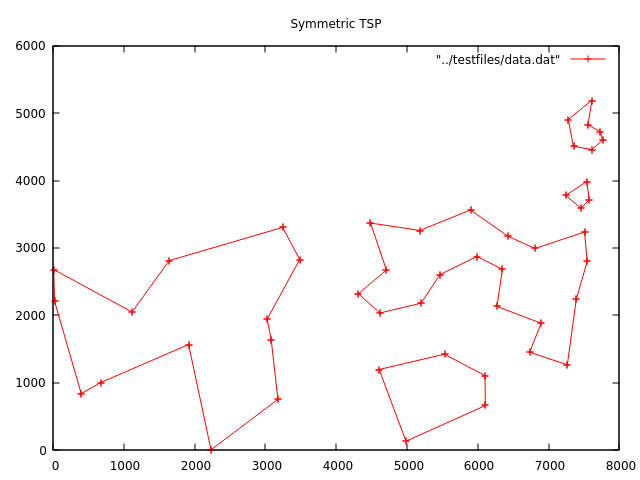
\includegraphics[width=0.6\textwidth]{images/symmetric_with_tours.png}
	\caption{The image represent att48.tsp solved with the problem formulation showed in section \ref{chapter:basic_model}}
	\label{fig:basic_model}
\end{figure}

Since sub-tours are present, this solution cannot be accepted. In the next sections SEC constraints will be added to the formula for avoiding this problem.

\section{The Miller, Tucker, and Zemlin model}
\label{chapter:mtz}
The model produced by Miller, Tucker, and Zemlin bypasses the exponential SECs by reducing their number to a simple polynomial.  Differently from the basic model, the graph obtained in this case is asymmetrical: $x_{ij}$ and $x_{ji}$ can have different weights.

In the new formulation, a new variable called $u_i$ is assigned to each node of the solution. This number represents an increasing sequence number in the optimal tour: starting from the second one ($u_2=0$), each node will increase the value by 1 at each following node until the end of the solution ($u_n=n-2$). The first node is considered special and its value is always set to $0$.

This is the new constraint added to the basic model by MTZ:
%\begin{comment}
	\begin{equation}
	\label{eqn:big-m}
	u_i-u_j+nx_{ij}\le n-1; \quad i,j\in \{2, \dots, n\}, i \not=j
	\end{equation}
	\begin{equation}
	\label{eqn:u-bound}
	0 \le u_i \le n-2; \quad integer \quad i \in V:i>1
	\end{equation}
%\end{comment}


The meaning of this formulation is the following: if the arc $x_{ij}$ is selected, then the value of $u_j$ is $u_j \ge u_i+1$ .

\subsection{Implementation of the model}
To express \ref{eqn:big-m} as a CPLEX constraint I need to rewrite the inequation in a way called Big-M. This method expects a new variable called $M$, which allows the system to activate or deactivate the constraint in a simple way. The new constraint will be:

\begin{equation}
\label{eqn:big-m-trick}
u_j\ge u_i+1-M(1-x_{ij})
\end{equation}

With this approach, the constraint is strictly depending on the value of $x_{ij}$. If $x_{ij}=1$, the constraint works like a normal one because the value of $M(1-x_{ij})$ will be $0$, so the meaning of \ref{eqn:big-m-trick} will be the same as the one expressed in the previous section. 
If $x_{ij}=0$, the right-hand side of the inequation will be certainly negative, making the constraint deactivated and allowing $u_j$ to take up any possible value from $0$ to $n-2$. Between all the values that $M$ can assume, the smallest one is $n-1$ due to the fact that, in the case of $X_{ij}=0$, the constraint will be still useful even if $u_i$ reaches its case limit of $n-2$.

With the application of the Big-M trick, the constraints can be written in the CPLEX environment. There are substantially 3 methods that can be implemented in the framework:

\begin{itemize}
	\item the use of standard constraints: all the constraints wrote in \ref{eqn:big-m} are directly saved into the problem at once. This lead to have $O(n^2)$ constraints active, making the optimization too large or even too expensive to solve;
	
	\item the use lazy constraints: as the name suggests, here the constraints are applied lazily. This means they are not always applied to the problem because CPLEX uses them only when necessary. In doing so, a pool of constraints is created and every time an integer optimal solution is found, the violation of every constraint in the pool is checked.
	If one of them is infringed, this constraint is added permanently to the instance. This method will hopefully make the problem smaller and faster to be solved than the one created with the standard constraints;
	
	\item the use of indicator constraints: in the first two cases the Big-M trick is used to trigger a constraint when a particular variable assumes a predetermined value, but this method is not always preferable since it can behave in unstable ways. That is why a good implementation of \ref{eqn:big-m} is the usage of the indicator constraints provided by the CPLEX API: this method automatically activates the constraint $u_j \ge u_i + 1$ when the $x_{ij}$ assumes the user passed value.
\end{itemize}

\section{The Gavish and Graves model}
The second compact model implemented is the one proposed by Gavish and Graves, based on the single commodity flow:  the arcs are considered as pipes.\\
Like in the MTZ model, a new variable is introduced in the problem. It is called "Flow of the arc" and it is represented with the symbol $y_{ij}$. Compared with the model in section \ref{chapter:mtz}, the starting value of $y_{ij}$ is $n-1$ and decrease by 1 at each following node in the optimal solution. 
To implement this proposition the following constraints are added to the model:
%\begin{comment}
\begin{equation}
\label{eqn:linking}
y_{ij}\le (n-1)x_{ij}
\end{equation}

\begin{equation}
\label{eqn:flow_first}
\sum_{j\in V;j\not=1}y_{1j}=n-1
\end{equation}

\begin{equation}
\label{eqn:flows}
\sum_{i, j\in V;i\not=j}y_{ij}-\sum_{j, k \in V;j\not=k}y_{jk}=1
\end{equation}
%\end{comment}

 

\clearpage{\pagestyle{plain}\cleardoublepage}
\chapter{Other sub-tour elimination methods} 
\label{chapter:other-sec} 
In chapter \ref{chapter:compact-models} I described models that cut out any possibility to have some sub-tours in the optimal solution. In this section I use particular techniques to remove the tours in a faster way.

\section{Benders method}
\label{chapter:benders}
This method is the simplest one presented in this chapter. The basic idea is the insertion of the SECs only when sub-tours are found. This is quite different from the implementation of the lazy constraints of MTZ seen before: the constraints are not activated when one of them is violated, but they are manually added into the instance.\\
This method uses the basic model described in \ref{chapter:basic_model} and follows this algorithm:

\begin{algorithm}
	\caption{Benders}\label{algo:benders}
	\begin{algorithmic}[1]
		\Require $G=(V,E), c:E\rightarrow \Re^+$
		\Ensure $z^*\text{ optimal solution}$
		\State instance $\gets$ *initializing basic model*
		
		\State successors, component$\gets$ *initialize arrays*
		\State ncomp $\gets$ 99999
		
		\While{$ncomp>1$}
			\State $z^*$ $\gets$ \textsc{CPXmipopt}
			\State successors, component, ncomp $\gets$ \textsc{build\_solution}($z^*)$
			\If{$ncomp > 1$}
				\State instance $\gets$ add violated constraints
			\EndIf	
		\EndWhile
		\State \Return $z^*$
	\end{algorithmic}
\end{algorithm}

This algorithm shows the simplicity of the Benders method. The first thing to do is building the basic model inside the instance of the CPLEX environment, and afterwards the arrays that will contain the successors and the components are initialized. These two arrays are $n$ long, so they are big enough to hold all the nodes. The most important function in this algorithm - excluded the optimization (\textsc{CPXmipopt}) - is the function \textsc{build\_solution}. It fills the arrays successors and components following this idea: search all the connected components inside the solution, then each $successors[i]$ will contain the next node inside the connected component, and $component[i]$ will enclose the index of the component of the node $i$. Then the algorithm checks the number of the connected components saved into ncomp. If more than one loop is present, the algorithm inserts a new constraint into the instance for each component, following this formula:
%\begin{comment}
\begin{equation}
\sum_{e\in E(S)}x_{e}\le |S|-1; \quad \forall S \subset\{2, \dots, n\}, \; |S|\ge 2
\end{equation}
%\end{comment}


where $E(S)$ are the edges contained inside the connected component $S$.

\section{Callback method}
\label{chapter:callback}
\section{Resolution with the callback method}
In sectio\ref{sec:problem-resolution} we introduce the fastest resolution method we've seen so far, but its implementation is a little bit tricky, and most of all not really "easthetic" CAMBIARE.\\
In this section we are going to explore the same loop method (so we will reject the solutions with some sub-tours) but this time we will implement its better version, also known as branch and cut.

\subsection{The callbacks}
Let's dive in in the main argument of this section: the callbacks.

As the name can suggest this type of function are not the classical one we have seen in section \ref{sec:setup} and \ref{sec:problem-resolution}, in fact every method of the callable library we have used is applied or before or after the optimization computed by CPLEX. The callback functions give to the user significant additional capabilities because they allow to intervene during the optimization, this upgraded abilities permit the user to work with the internal data structure of CPLEX so the developer must be aware of what he is doing.

CPLEX has three different types of callbacks: informational callbacks, query/diagnostic callbacks, and control callbacks. The first ones gives the user additional information on the current optimization without affection the performance or interfering with the solution search space. The second ones access to more detailed informations respect to the informational callbacks but can affect the overall performance of the problem resolution; the query/diagnostic callbacks are also incompatible with the dynamic search and deterministic parallel functions. The last ones are the one we are going to use and they allow the user to alter and customize how CPLEX perform the optimization.

In order to use them we need to declare their usage before calling the optimization function, we can do this through the function of the callable library:

\begin{lstlisting}
	CPXcallbacksetfunc(env, lp, CPX_CALLBACKCONTEXT_CANDIDATE, sec_callback, inst)
\end{lstlisting}

In this piece of code we can see the variables \verb|env| and \verb|lp| are the well known environment and problem of CPLEX. The third argument (\verb|CPX_CALLBACKCONTEXT_CANDIDATE|) is what the API documentation call contextmask, usually this value must be one of the constants described the callable library; the value passed in the function tells CPLEX to call the callback function (the fourth argument, \verb|sec_callback|) everytime it finds an integer solution of the problem. The last argument is the user data that are passed to the callback function.


\subsection{Callback with an integer solution}
The first callback we analyze are the one that will be called when CPLEX finds an integer solution. Once the function is called we can perform some operations with the informations we can retrieve from the problem. The operations we perform are similar to the ones descripted in section \ref{sec:sol_management}.

First we retrieve the solution found by CPLEX with the function \verb|CPXcallbackgetcandidatepoint|, than we perform the same operations we have done when we described the \verb|build_solution| function, so we find all the components of the solution. When there are more than one componentes, so some sub-tours are present, we add to the problem the reason why the solution is infeasable for us through the function \verb|CPXcallbackrejectcandidate|. The meaning of the function is that the current solution found during the optimization is not feasable since it violetes the costraints that we pass as arguments (in fact are similar to the one used when we used the lazy constraints in the MTZ model).

\subsection{Callback with a fractional solution}
The management of this solutions are really more complex than the one previously analyzed since as all the values in the solution are not integer so we can't handle as we have done before (with the method of the components). Because the operations to perform in order to compute if the solution is composed by sub-tours we decided to use an external static library called \href{https://www.math.uwaterloo.ca/tsp/concorde.html}{Concorde}.
This library is one of the most powerful available in the market, it has even its own iOS application that allow to solve pretty complex instance of the problem.

The problem with this kind of solution its that can contains some nodes where the number of incidence edges is greater that 2 but their values are weighted in such way to respect anyway the degree costraint.

The methods appleid by Concorde to solve the fractional problem require that the graph is connected (using the function \verb|CCcut_connect_components|), if its true we can call another function that allow us to implement the addition of a cut to the problem (performed by \verb|CPXcallbackaddusercuts|).

\subsection{Performance Analysis}
SCIRVERE QUI LE PERFEORMANCE

%Spiegare il funzionamento 

\subsection{Callback on the fractional solutions}
\label{chapter:callback-fractional}
In the previous section, the callback was called on each integer candidate solution. This sector will describe the use of the callback even on the fractional solution.\\
The object of this idea is to save computational time by adding new SECs that are probably common in the decision tree. The procedure defined in this phase is the same in section \ref{chapter:callback}, except that this callback is applied in the continuous relaxation of the problem.
To implement this kind of operation I used an external library called Concorde \cite{concorde}. This library is written in ANSI C and is one of the most powerful tool on the market: it can solve really large instances of the TSP problem to the optimal solution.\\
When the callback is called I use the library mentioned above to compute which SEC I require to exclude the fractional solution from the decision tree. 

\clearpage{\pagestyle{plain}\cleardoublepage}
\chapter{Non optimal solutions} 
\label{chapter:codice} 
In this section I am going to explore a new branch of the TSP resolution. Now the discovery of an optimal solution is no longer important. This can be achieved through the use of the matheuristic and heuristic to find a solution, with a great approximation to the optimal one, even with instances including millions of nodes. In this chapter I am going to cover different approach such as: matheuristic methods, heuristic and metaheuristic algoritms.


\section{Matheuristics}
"The objective of a heuristic is to produce a solution in a reasonable time frame that is good enough for solving the problem at hand. This solution may not be the best of all the solutions to this problem, or it may simply approximate the exact solution. But it is still valuable because finding it does not require a prohibitively long time"\cite{heuristic}.\\
The two techniques I am going to delve into are the hard-fixing and the soft-fixing.

\subsection{Hard-fixing}
\label{section:hard-fix}
The main purpose of this method is to try to reduce the search space by cutting down the complexity of the optimization. For achieving this goal, an initial feasible solution is needed - obtained by any approach described in this report.\\
The central thought of hard-fixing is to get an easier problem by setting some variables of the solution passed to the method - and so by having fewer variables to compute. The variables to be fixed are $x_{ij}$, $i, j\in V$. This task is done by settling the values to 1, so that the edge will be surely part of the solution. A valid method to choose which path is designated to be fixed is to link each edge to a probability $p$ between $0$ and $1$, then set randomly - with the probability picked - the value to 1.\\
Hereupon, the problem will presumably have $p*|E|$ variables fixed and thus the instance can be solved with a lower effort. Hopefully, this situation will bring to a better solution. Although the choice of using a probability is a good pick, any other method can be used to block the edges.

The performance of this technique is strictly related to the choice of the first feasible solution: if it is not good enough, this approach will get stuck on some non-optimal solution. A good fix for avoiding this is to lower down $p$ whenever the solution is not improved for a predetermined amount of time.

\begin{algorithm}
	\caption{Hard-fixing}\label{algo:hard-fix}
	\begin{algorithmic}[1]
		\Require $G=(V,E)$,$ c:E\rightarrow \Re^+$, $global\_timelimit$, $iteration\_timelimit$
		\Ensure $z\text{ hopefully good solution}$
		\State instance $\gets$ *initializing model (any of this report)*
		
		\State  $z$ $\gets$ \textsc{CPXmipopt} *with nodelimit 0*
		\State $p$ $\gets$ $0.9$
		\State $i$ $\gets$ $0$
		\While{$time\_elapsed<global\_time\_limit$}
			\If{$time\_remaining > iteration\_timelimit$}
				\State instance $\gets$ *set timelimit to $iteration\_timelimit$*
			\Else 
				\State instance $\gets$ *set timelimit to $time\_remaining$*
			\EndIf
			\State instance $\gets$ *hard-fixing with probability $p$*
			\State $z_{new}$ $\gets$ \textsc{CPXmipopt}
			
			\If{$cost(z_{new})<cost(z)$}
				\State $z$ $\gets$ $z_{new}$
				\State $i$ $\gets$ $0$
			\Else 
				\State $i$ $\gets$ $i+1$
			\EndIf
			
			\If{$i = 10$}
				\State $p$ $\gets$ $p - 0.1$
			\EndIf
			\State instance $\gets$ *remove hard-fixing*
		\EndWhile
		\State \Return $z$
	\end{algorithmic}
\end{algorithm}

In this algorithm, there are some variables not mentioned before: the global timelimit and the iteration timelimit. As aforementioned, the hard-fixing is a technique that aims to obtain a good solution in a short amount of time, so the parameters described above are necessary to establish - as the name suggests - the timespan in which the optimization is solved. global\_timelimit is the total time reserved to the solver, interation\_timelimit is the duration of each optimization in which the hard-fixing is applied.

The initial solution is provided by the solver, limited in the depth of its analysis. Then, algorithm \ref{algo:hard-fix} starts to iterate the main process until the global\_timelimit is reached. During this phase, the optimization is called several times, in each of which the instance is solved blocking some variables to $1$.

\subsection{Soft-fixing}
The technique that will be described is called Local Branching. Since it is a slight modification of the hard-fixing it is also called soft-fixing.\\
In section \ref{section:hard-fix} the value of the variables is fixed in a manual way using a probability system. In Local Branching, this operation is performed by adding a new constraint that forces the instance to block a predetermined number of variables, giving to the solver a degree of freedom on which variables to fix and which not.

The main idea of soft-fixing is the Hamming distance: "it measures the minimum number of substitutions required to change one string into the other"\cite{hamming-distance}. This description can be applied also to vectors. So given two vectors $x$ and $\tilde{x}$ in $\{0,1\}$, the Hamming distance is the number of different bits they have. It can be described in this way:

\begin{equation}
\label{eqn:hamming-dist}
H(x, \tilde{x}) = \sum_{j:\tilde{x}_j=1}(1-x_j)+\sum_{j:\tilde{x}_j=0}x_j
\end{equation}

Considering that the output solution of the solver is a vector in $\{0, 1\}$, it is possible to insert into the instance a new constraint that limits the hamming distance between the old solution and the new one.
The number of edges active in each solution is forced to be $n=|V|$ and therefore the Hamming distance is computed on the differences in the bits equal to 1. For this reason, it is possible to reduce \ref{eqn:hamming-dist} to:

\begin{equation}
\label{eqn:hamming-dist-2}
H(x, \tilde{x}) = \sum_{j:\tilde{x}_j=1}(1-x_j) =  n - \sum_{j:\tilde{x}_j=1}x_j
\end{equation}

The purpose of this method is to limit the diversity of two solutions. For doing so, it is possible to add a new variable $k$ that limits the Hamming distance. Through elementary math, this formulation is built as:

\begin{equation}
\label{eqn:hamming-dist-3}
H(x, \tilde{x}) \le k \Rightarrow n - \sum_{j:\tilde{x}_j=1}x_j \le k \Rightarrow \sum_{j:\tilde{x}_j=1}x_j \ge n - k
\end{equation}

The consequence of \ref{eqn:hamming-dist-3} is to narrow the next iteration of the optimization to a $k$-neighborhood of the previous one. As the method described in section \ref{section:hard-fix}, the value $k$ can vary if for the optimization doesn't improve the solution. 

\begin{algorithm}
	\caption{Soft-fixing}\label{algo:soft-fix}
	\begin{algorithmic}[1]
		\Require $G=(V,E)$,$ c:E\rightarrow \Re^+$, $global\_timelimit$, $iteration\_timelimit$
		\Ensure $z\text{ hopefully good solution}$
		\State instance $\gets$ *initializing model (any of this report)*
		
		\State  $z$ $\gets$ \textsc{CPXmipopt} *with nodelimit 0*
		\State $k$ $\gets$ $2$
		\State $i$ $\gets$ $0$
		\While{$time\_elapsed<global\_time\_limit$}
		\If{$time\_remaining > iteration\_timelimit$}
		\State instance $\gets$ *set timelimit to $iteration\_timelimit$*
		\Else 
		\State instance $\gets$ *set timelimit to $time\_remaining$*
		\EndIf
		\State instance $\gets$ *soft-fixing using a k-neighborhood*
		\State $z_{new}$ $\gets$ \textsc{CPXmipopt}
		
		\If{$cost(z_{new})<cost(z)$}
		\State $z$ $\gets$ $z_{new}$
		\State $i$ $\gets$ $0$
		\Else 
		\State $i$ $\gets$ $i+1$
		\EndIf
		
		\If{$i = 10$}
		\State $k$ $\gets$ $k + 1$
		\EndIf
		\State instance $\gets$ *remove soft-fixing*
		\EndWhile
		\State \Return $z$
	\end{algorithmic}
\end{algorithm}

The only changes between \ref{algo:hard-fix} and \ref{algo:soft-fix} are the variables used and the constraints added to the instance. In this implementation, $k$ is increased by $1$ every time the solution is not improved.

\section{Heuristics}
In this section the concept of heuristic is explored in some of algorithms used to solve the TSP problem. In particular, a set of methods will be presented namely greedy algorithm, extra mileage, and 2-opt optimization.

\subsection{Greedy algorithm}
\label{sec:greedy}
This type of method is the easiest to understand and implement. This heuristic has its roots on the concept  of constructing the shortest path by connecting the nearest nodes.

This algorithm starts from an arbitrary node and chooses its following node by selecting the nearest one from the ones that are not already in the path. For this reason, it is also called Nearest Neighbor.

The main side effect is that the shortest path is easily missed since the last nodes - apart from special cases - are far from each othe and in this way the optimal solution is not selected. The algorithm is the following: 

\begin{algorithm}
	\caption{Greedy}\label{algo:greedy}
	\begin{algorithmic}[1]
		\Require $G=(V,E)$,$ c:E\rightarrow \Re^+$
		\Ensure $z\text{ hopefully good solution}$
		\State $best\_cost$ $\gets$ $+\infty$
		\State $z$ $\gets$ *empty*
		
		\For{$start\_node$ $\gets$1 $to$ n}
			\State $current\_node$ $\gets$ $start\_node$
			\While{*each node is visited*}
			\State $candidate\_node \gets$ $-1$
				\For{$i \gets 1$ $to$ n}
					\State *Finds the nearest node and marks it as visited*
					\State $candidate\_node \gets$ *nearest node*
				\EndFor
				\State *Saves $candidate\_node$ as next node*
				\State $current\_node$ $\gets$ $candidate\_node$
			\EndWhile
			\If{cost($z_{curr}$)$<best\_cost$}
				\State $best\_cost$ $\gets$ $cost(z_{curr})$
				\State $z$ $\gets$ $z_{curr}$
			\EndIf
		\EndFor
		\State \Return $z$
	\end{algorithmic}
\end{algorithm}

The classic implementation has a complexity of $O(n^2)$ since each node has to search the nearest node all over the graph. To obtain the best solution possible, in my implementation each node is tested as starting node. In particular, \ref{algo:greedy} has a complexity of $O(n^3)$ because of the aforementioned method to select the best starting node.\\
This complexity is quite low but it can be slower than expected with some instances over a great number of nodes.

\subsection{Extra mileage approach}
\label{sec:extra-mileage}
This approach is more complex than the previous one but in favor of a better solution. The main idea behind this algorithm is very simple and it sets up from an empty solution.

It starts by connecting the farthest nodes in the instance with a cycle, and this path will be the beginning of the solution. Then, the closest node among the active edges is selected and added to the solution by replacing it with two more edges that allow the new node to enter the solution. This process can be seen in figure \ref{fig:extra}, where it is performed with a five nodes.

\begin{figure}
	\centering
	\begin{subfigure}[b]{0.3\textwidth}
		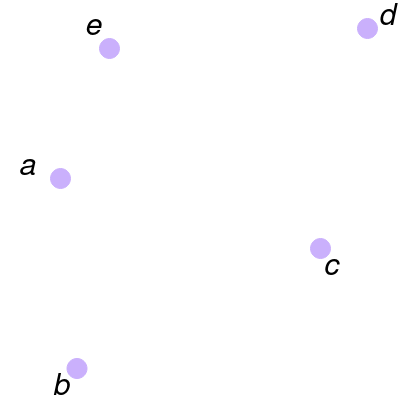
\includegraphics[width=\textwidth]{images/extra_1}
		\caption{No edges}
	\end{subfigure}
	\hfill
	\begin{subfigure}[b]{0.3\textwidth}
		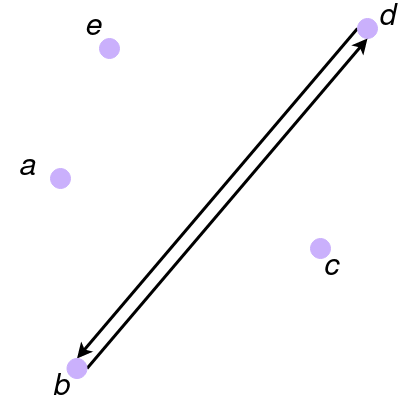
\includegraphics[width=\textwidth]{images/extra_2}
		\caption{First two edges added}
	\end{subfigure}
	\hfill
	\begin{subfigure}[b]{0.3\textwidth}
		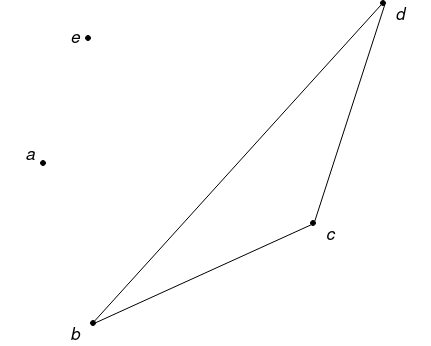
\includegraphics[width=\textwidth]{images/extra_3}
		\caption{One edge is substituted with other two connecting one more node}
	\end{subfigure}
	\bigskip
	\begin{subfigure}{0.3\textwidth}
		\centering
		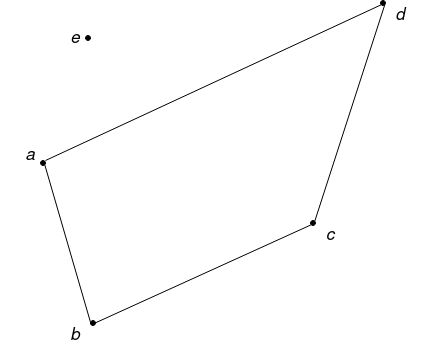
\includegraphics[width=\textwidth]{images/extra_4}
		\caption{Added one more node}
	\end{subfigure}
	\hfill
	\begin{subfigure}{0.3\textwidth}
		\centering
		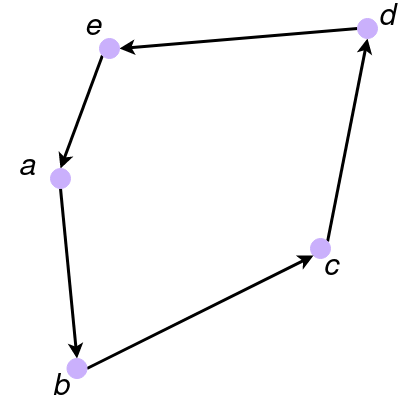
\includegraphics[width=\textwidth]{images/extra_5}
		\caption{All nodes are connected}
	\end{subfigure}
	\caption{In this image we can see the process done by extra-mileage to find the solution.}
	\label{fig:extra}
\end{figure}

For inserting the next node, the method used is the triangle inequality, which states that the sum of the lengths of any two sides must be greater than or equal to the length of the remaining side. In doing so with the replacing phase, some cost is added to the solution. Imagine taking into consideration three nodes $x$, $y$ and $z$, where $x$ and $y$ are already in the solution and $z$ wants to join them. The mathematical operation to apply is the following:

\begin{equation}
	\Delta(x, y, w) = c_{xw} + c_{yw} - c_{xy}
\end{equation}

This value will always be positive thanks to the aforementioned triangle inequality.

The algorithm used is the following:
\begin{algorithm}
	\caption{Extra mileage}\label{algo:extra-mileage}
	\begin{algorithmic}[1]
		\Require $G=(V,E)$,$ c:E\rightarrow \Re^+$
		\Ensure $z\text{ hopefully good solution}$
		\State $x, y$ $\gets$ *finds the farthest nodes*
		\State $z$ $\gets$ \textsc{Add($x, y$)}
		
		\While{$|z|<n$}
			\State $(x, y, w)$ $\gets$ argmin($\Delta(x, y, w):x, y \in z, w \not \in z$)
			\State $z$ $\gets$ \textsc{Add($w $)}
		\EndWhile
		\State \Return $z$
	\end{algorithmic}
\end{algorithm}

\subsection{2-opt refining}
This section analyzes a refining technique where the goal is to take an existing solution $x$ and to put it closer to the optimum one.\\
The $k$-opt refining consists on rearrange $k$ edges in order to obtain a new solution with a lower cost. In particular, this section describes the $2$-opt refining.

To handle this approach effectively, it is applied starting from a solution obtained with a heuristic approach - such as the ones described in section \ref{sec:greedy} and \ref{sec:extra-mileage}. The idea of this algorithm is to remove all the crossing edges and to insert new edges that will decrease the cost of the final solution.

Here too the triangle inequality is used to find the couple of edges that allow the best improvement. In this implementation, the operation is done across four nodes: $i$, $succ[i]$, $j$, and $succ[j]$. Since the tour is asymmetric, it has a direction: $succ[i]$ and $succ[j]$ are respectively the following nodes in the path of the nodes $i$ and $j$. 

\begin{equation}
	\label{eqn:2-opt}
	\Delta (i, j) = (c_{i, succ[i]} + c_{j, succ[j]}) - (c_{i, j} + c_{succ[i], succ[j]}) \quad i, j \in V; i\not=succ[j]; j\not=succ[i]
\end{equation}

In \ref{eqn:2-opt} it is described the correct way to compute the delta of the method. Greater the value, better the improving.

\begin{figure}[h]
	\centering
	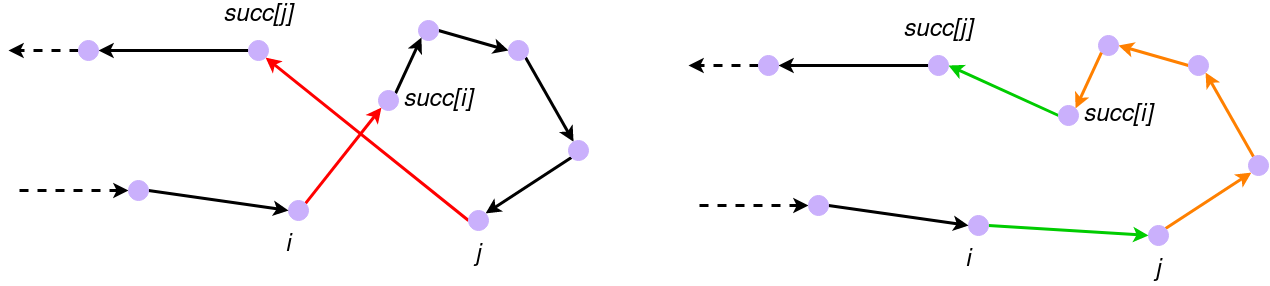
\includegraphics[width=0.9\textwidth]{images/2_opt_new.png}
	\caption{The image represent the replacement of two edges during the $2$-opt refining.}
	\label{fig:2-opt}
\end{figure}

In figure \ref{fig:2-opt} it is possible to look at the replacement of two arcs. It is important to notice that the path from $i$ to $succ[i]$ changes direction after the substitution of the old edges. This is done for maintaining the solution integrity. In particular, this optimization is performed until no more positive $\Delta(i, j)$ are found. If they are not found, the solution is no more improvable by the 2-opt algorithm.

\begin{algorithm}
	\caption{$2$-opt refining}\label{algo:2-opt}
	\begin{algorithmic}[1]
		\Require $G=(V,E)$,$ c:E\rightarrow \Re^+$
		\Ensure $z\text{ hopefully good solution}$
		\State $z$ $\gets$ *find feasible solution with an algorithm*
		\State flag $\gets$ $false$
		
		\While{$flag==false$}
			\State flag $\gets$ $true$
			\State $(i, j)$ $\gets$ argmax($\Delta(i, j):i, j\in V)$
			\If{$\Delta(i, j)>0$}
				\State flag $\gets$ $false$
				\State $z$ $\gets$ *edge replacement*
			\EndIf
		\EndWhile
		\State \Return $z$
	\end{algorithmic}
\end{algorithm}

\begin{figure}
	\centering
	
	\begin{subfigure}[b]{0.45\textwidth}
		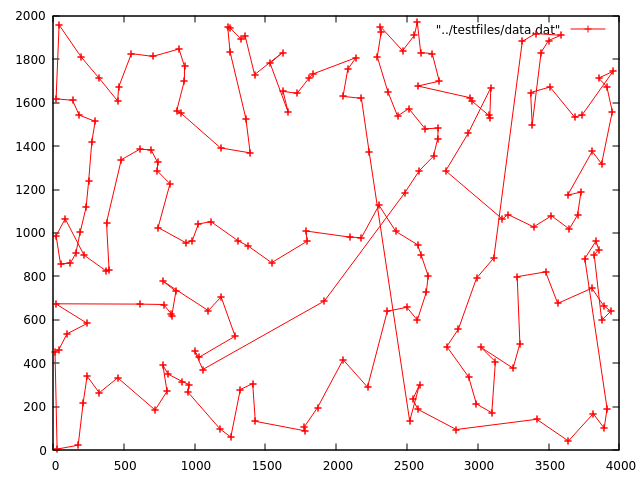
\includegraphics[width=\textwidth]{images/kroA_greedy.png}
	\end{subfigure}
	\hfill
	\begin{subfigure}[b]{0.45\textwidth}
		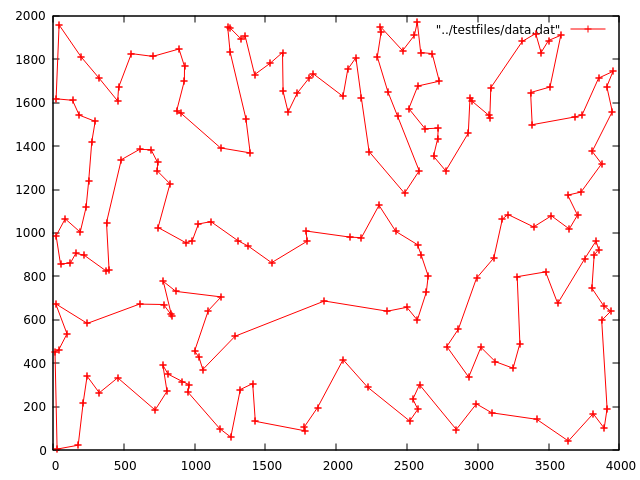
\includegraphics[width=\textwidth]{images/2_opt.png}
	\end{subfigure}
	\caption{The improvement obtained applying to a greedy algorithm (left) the 2-opt refining approach (right).}
\end{figure}

\section{Metaheuristics}
\label{chapter:metaheuristics}
While the heuristic approach seen before was strictly specific to the TSP problem, the concept of metaheuristic is quite different. Their procedure is problem-independent and does not take advantage of any specificity of the problem. Generally, these techniques are not greedy and can accept a temporary deterioration of the solution in order to have a bigger search space in which to find a better solution.

In this section, some of them will be used such as the variable neighborhood search and the tabu search.

\subsection{Variable Neighborhood Search}
\label{sec:VNS}
The variable neighborhood search (VNS) is the first metaheuristic approach presented. Its main purpose is to try to escape from a local optimal of the solution aiming to find the optimal solution of the problem. 

The instance of the problem can be seen as a function with its local minima, local maxima, and so on. During the utilization of some heuristic techniques, it is possible that the process remains stuck in a sub-optimal area. The way in which it tries to escape from this region is done by changing the \textit{neighborhood} of the solution: some data are modified and then a new minimum is searched.

In this report, the adjustment of the neighborhood is performed by a perturbation phase in which is applied a $k$-opt kick. This change is performed by selecting randomly a $k$ set of edges and then replacing them with others in order to obtain a poor solution. In particular, the procedure done is the following: a $2$-opt refining is applied to a reference solution, once the minimum is reached a kick is given to the solution to worsening the solution. Then the $2$-opt refining approach is used again to find a new minimum. In my implementation are implemented three perturbations: 3, 5, and 7. An example of implementation can be seen in Algorithm \ref{algo:vns}.

\begin{algorithm}
	\caption{VNS}\label{algo:vns}
	\begin{algorithmic}[1]
		\Require $G=(V,E)$,$ c:E\rightarrow \Re^+, k, global\_timelimit$
		\Ensure $z\text{ hopefully good solution}$
		\State $z_{curr}$ $\gets$ $z$ $\gets$ *built solution using an heuristc*
		\State $best\_cost$ $\gets$ cost($z$)
		\State cycles $\gets$ $0$
		\While{$time\_elapsed<global\_timelimit$}
			\State $z_{curr}$ $\gets$ \textsc{2-opt($z_{curr}$)}
			\If{cost($z_{curr}$) $< best\_cost$}
				\State z $\gets$ $z_{curr}$
				\State $best\_cost$ $\gets$ cost($z_{curr}$)
			\EndIf
		\State *Bigger the value of cycles bigger the kick*
		\State $z_{curr}$ $\gets$ \textsc{k-kick($cycles$)}
		\State cycles $\gets$ cycles$+1$
		\EndWhile
		\State \Return $z$
	\end{algorithmic}
\end{algorithm}


\subsection{Tabu search}
\label{sec:tabu-search}
The tabu search is the second metaheuristic presented in this report. It is a method to improve the local search and avoid falling back in a previous local minimum. To do that the concept of tabu is introduced: a set of banned solutions prevents the algorithm to return an already visited result.

In this implementation of the tabu search the refining phase is performed by a 2-opt move as it happened in section \ref{sec:VNS}, then the method to escape from this minimum is to perform a kick like as the previous section. The main difference is that during the VNS is possible to fall again and again in the previous solution, using the tabu search is not possible. 

The worsening move is performed by swapping two non-consecutive edges, then they are declared as tabu: they cannot be swapped for a while. This process precludes the possibility of falling into a cycle of deterioration-recover, where to final solution is always the same. This algorithm will continuously worsen the solution until a non-tabu move is performed.

The way in which this method is implemented is the following: each time a worsening action is performed the nodes selected are declared as tabu and the edges connected with them cannot be changed by any improving moves. If each time this action has been performed the list of tabu nodes becomes so large that no more moves are allowed. To avoid this case it is introduced a new variable called $tenure$, its main idea is to limit how many times a tabu is valid.

To do that we declare a node tabu (for example $i$) by inserting into an array the iteration number $h$, so $tabu\_nodes[i] = h$. This constraint will last for a $tenure$ number of times, following this rule:

\begin{equation}
	iteration\_number - tabu[i] \le tenure
\end{equation}

A good choice of $tenure$ is crucial to allow the algorithm to perform adequately. The best decision is to make it variable regarding the number of iterations already completed. In algorithm \ref{algo:tabu-search} can be seen the proceeding of this method.

\begin{algorithm}
	\caption{Tabu search}\label{algo:tabu-search}
	\begin{algorithmic}[1]
		\Require $G=(V,E)$,$ c:E\rightarrow \Re^+, k, global\_timelimit$
		\Ensure $z\text{ hopefully good solution}$
		\State $z_{curr}$ $\gets$ $z$ $\gets$ *built solution using an heuristc*
		\State $best\_cost$ $\gets$ cost($z$)
		\State $iteration\_counter \gets 1$
		\While{$time\_elapsed<global\_timelimit$}
			\State *Performs a 2-opt refining applying the constaraint described in section \ref{sec:tabu-search}. The iteration counter is increased each time a move is performed. If no moves are allowed this method does nothing*
			\State $z_{new}$ $\gets$ \textsc{tabu-2-opt($z_{curr}, tabu, tenure, iteration\_counter$)}
			\If{cost($z_{curr}$) $< best\_cost$}
				\State z $\gets$ $z_{curr}$
				\State $best\_cost$ $\gets$ cost($z_{curr}$)
			\EndIf
			\State $first\_node \gets RANDOM(|V|)$
			\State $second\_node \gets RANDOM(|V|)$
			\State $tabu[first\_node] \gets iteration\_counter$
			\State $tabu[second\_node] \gets iteration\_counter$
			\State $z_{curr} \gets $ \textsc{2-kick($first\_node, second\_node$)}
			\State $iteration\_counter \gets iteration\_counter+1$
		\EndWhile
		\State \Return $z$
	\end{algorithmic}
\end{algorithm}

\subsection{Genetic algorithms} 

\clearpage{\pagestyle{plain}\cleardoublepage}
\begin{thebibliography}{99}
\addcontentsline{toc}{chapter}{Bibliografia}


\bibitem{ro1} Fischetti M., \textit{Lezioni di Ricerca Operativa}, Aprile 2018.

\bibitem{concorde} \textit{Concorde TSP Solver}, \url{https://www.math.uwaterloo.ca/tsp/concorde.html}, last consultation: 02/02/2022.

\bibitem{heuristic} \textit{Heuristic (computer science)}, \url{https://en.wikipedia.org/wiki/Heuristic_(computer_science)}, last consultation: 02/02/2022.

\bibitem{hamming-distance} \textit{Hamming distance}, \url{https://en.wikipedia.org/wiki/Hamming_distance}, last consultation: 05/02/2022.


\end{thebibliography}


\end{document}
